%%%%%%%%%%%%%%%%%%%%%%%%%%% asme2e.tex %%%%%%%%%%%%%%%%%%%%%%%%%%%%%%%%%%%%%%%%%%%%
% Template for producing Ph. D dissertation using LaTeX                           %
% Written by   Marco Longhitano and Stefan Jeske                                  %
%              Istitute for Fluid Power Drives and Controls (IFAS)                %
%              RWTH University Aachen                                             %
%              Steinbachstrasse 53                                                %
%              D-52074 Aachen                                                     %
%              Tel: (+49) 0241 - 80 27525 (0ffice)                                %
%              Email: marco.longhitanoqifas.rwth-aachen.de                        %
%              WWW:   http://www.ifas.rwth-aachen.de/                             % 
%              April 1, 2016                                                      %
% Modified:                                                                       %
% Use at your own risk, send complaints to marco.longhitano@ifas.rwth-aachen.de   %
%%%%%%%%%%%%%%%%%%%%%%%%%%%%%%%%%%%%%%%%%%%%%%%%%%%%%%%%%%%%%%%%%%%%%%%%%%%%%%%%%%%

%Classes abd Styles
\documentclass{Classes/ifasDiss}
\usepackage{Styles/ifasDissMacros}
\usepackage{lipsum}

%turn off those nasty overfull and underfull hboxes
\hbadness=10000
\hfuzz=50pt

%Info for the pdf file
\ifpdf
    \pdfinfo { /Title  (IFAS Dissertation Template in Latex)
               /Creator (TeX)
               /Producer (pdfTeX)
               /Author (Marcus Tullius Cicero)
               /CreationDate (D:20160321000000)  %format D:YYYYMMDDhhmmss
               /ModDate (D:20160322000000)
               /Subject (Writing a PhD thesis in LaTeX)
               /Keywords (PhD, Thesis)}
    \pdfcatalog { /PageMode (/UseOutlines)
                  /OpenAction (fitbh)  }
\fi

%Info about author and document(used for the titlepage)
\author{Marcus Tullius Cicero}
\title{IFAS Dissertation Template in Latex}
\secondCorrector{Name}
\dateOfExam{Date}

\begin{document}
%Titlepage
\maketitle

\frontmatter
%Dedication
\begin{dedication}
I love tube socks!\\ --{\scshape Miley Cyrus}
\end{dedication}

%Acknowledgement
\begin{acknowledgement}
First of all, I would like to thank Milos for his support. A special thank goes to Milos as well. Finally, I cannot forget to thank Milos. First of all, I would like to thank Milos for his support. A special thank goes to Milos as well. Finally, I cannot forget to thank Milos. First of all, I would like to thank Milos for his support. A special thank goes to Milos as well. Finally, I cannot forget to thank Milos. First of all, I would like to thank Milos for his support. A special thank goes to Milos as well. Finally, I cannot forget to thank Milos. First of all, I would like to thank Milos for his support. A special thank goes to Milos as well. Finally, I cannot forget to thank Milos. First of all, I would like to thank Milos for his support. A special thank goes to Milos as well. Finally, I cannot forget to thank Milos. First of all, I would like to thank Milos for his support. A special thank goes to Milos as well. Finally, I cannot forget to thank Milos. First of all, I would like to thank Milos for his support. A special thank goes to Milos as well. Finally, I cannot forget to thank Milos. First of all, I would like to thank Milos for his support. A special thank goes to Milos as well. Finally, I cannot forget to thank Milos. First of all, I would like to thank Milos for his support. A special thank goes to Milos as well. Finally, I cannot forget to thank Milos. First of all, I would like to thank Milos for his support. A special thank goes to Milos as well. Finally, I cannot forget to thank Milos. First of all, I would like to thank Milos for his support. A special thank goes to Milos as well. Finally, I cannot forget to thank Milos. First of all, I would like to thank Milos for his support. A special thank goes to Milos as well. Finally, I cannot forget to thank Milos.  
\end{acknowledgement}

%Zusammenfassung/Abstract
\begin{abstract}
In english in english in english in english in english in english in english in english in english in english in english in english in english in english in english in english in english in english in english in english in english in english in english in english in english in english in english in english in english in english in english in english in english in english in english in english in english in english in english in english in english in english in english in english in english in english in english in english in english in english in english in english in english in english in english in english in english in english in english in english in english in english in english in english in english in english in english in english in english in english in english in english in english in english in english in english in english in english in english in english in english in english in english in english in english in english in english in english in english in english in english in english in english in english in english in english in english in english in english in english in english in english in english in english in english in english in english in english in english in english in english in english in english in english in english in english in english in english in english in english in english in english in english in english in english in english in english in english in english in english in english in english in english in english in english in english in english in english in english in english in english in english in english in english in english in english in english in english in english in english in english in english in english in english in english in english in english in english in english in english in english in english in english in english in english in english in english in english in english in english in english in english in english in english in english in english in english in english in english in english in english in english in english in english in english in english in english in english in english in english in english in english in english in english in english in english in english in english in english in english in english in english in english in english in english in english in english in english in english in english in english in english in english in english in english in english in english in english in english in english in english in english in english in english in english in english in english in english in english in english in english in english in english in english in english in english in english in english in english in english in english in english in english in english in english in english in english in english in english in english in english. 
\newpage\thispagestyle{empty} %To comment in case of two pages abstract
\null %To comment in case of two pages abstract
%Please avoid an abstract larger than 1 page
\end{abstract}
\begin{zusammenfassung}
Auf deutsch  auf deutsch auf deutsch auf deutsch auf deutsch auf deutsch auf deutsch auf deutsch auf deutsch auf deutsch auf deutsch auf deutsch auf deutsch auf deutsch auf deutsch auf deutsch auf deutsch auf deutsch auf deutsch auf deutsch auf deutsch auf deutsch auf deutsch auf deutsch auf deutsch auf deutsch auf deutsch auf deutsch auf deutsch auf deutsch auf deutsch auf deutsch auf deutsch auf deutsch auf deutsch auf deutsch auf deutsch auf deutsch auf deutsch auf deutsch auf deutsch auf deutsch auf deutsch auf deutsch auf deutsch auf deutsch auf deutsch auf deutsch auf deutsch auf deutsch auf deutsch auf deutsch auf deutsch auf deutsch auf deutsch auf deutsch auf deutsch auf deutsch auf deutsch auf deutsch auf deutsch auf deutsch auf deutsch auf deutsch auf deutsch auf deutsch auf deutsch auf deutsch auf deutsch auf deutsch auf deutsch auf deutsch auf deutsch auf deutsch auf deutsch auf deutsch auf deutsch auf deutsch auf deutsch auf deutsch auf deutsch auf deutsch auf deutsch auf deutsch auf deutsch auf deutsch auf deutsch auf deutsch auf deutsch auf deutsch auf deutsch auf deutsch auf deutsch auf deutsch auf deutsch auf deutsch auf deutsch auf deutsch auf deutsch auf deutsch auf deutsch auf deutsch auf deutsch auf deutsch auf deutsch auf deutsch auf deutsch auf deutsch auf deutsch auf deutsch auf deutsch auf deutsch auf deutsch auf deutsch auf deutsch auf deutsch auf deutsch auf deutsch auf deutsch auf deutsch auf deutsch auf deutsch auf deutsch auf deutsch auf deutsch auf deutsch auf deutsch auf deutsch auf deutsch auf deutsch auf deutsch auf deutsch auf deutsch auf deutsch auf deutsch auf deutsch auf deutsch auf deutsch auf deutsch auf deutsch auf deutsch auf deutsch auf deutsch auf deutsch auf deutsch auf deutsch auf deutsch auf deutsch auf deutsch auf deutsch auf deutsch auf deutsch auf deutsch auf deutsch auf deutsch auf deutsch auf deutsch auf deutsch auf deutsch auf deutsch auf deutsch auf deutsch auf deutsch auf deutsch auf deutsch auf deutsch auf deutsch auf deutsch auf deutsch auf deutsch auf deutsch auf deutsch auf deutsch auf deutsch auf deutsch auf deutsch auf deutsch auf deutsch auf deutsch auf deutsch auf deutsch.
\newpage\thispagestyle{empty} %To comment in case of two pages zusammenfassung
\null %To comment in case of two pages zusammenfassung
%Please avoid an zusammenfassung larger than 1 page
\end{zusammenfassung}
 
%Reset Pagenumbering to 1 and small romans
\pagenumbering{roman}

%Print Table of contents
\tableofcontents

%Add the Nomenclature to the toc
%Use 
% <makeindex dissertationTemplate.nlo -s nomencl.ist -o dissertationTemplate.nls>
%to add new entries to the nomenclature. Afterwards compile .tex again
\setlength{\nomitemsep}{-0.5ex}%Interline
\printnomenclature[6em]%Intercolumn

%Start mainmatter
\mainmatter
\pagestyle{mainmatter}

\chapter{Introduction}
\lipsum[1-8] 

\chapter{Fundamentals}
\section{First Section Name}
\lipsum[1-7]

\section{Second Section Name}
\subsection{Subsection Name}
\lipsum[1-4]

\subsubsection{It does not appear in contents}
\lipsum[1-2]

\section{Figures, Equations, Nomenclature and Reference}
\nomwithunits{R}{\(a,b,c\)}{half axes of ellipsoid}{\si{m}}%Example of nomenclature
\nomwithunits{G}{$\sigma$}{Surface Tension}{\si{F.m^{-2}}}%
\nomwithunits{R}{\(C\)}{dimensionless coefficient (e.g.\ for drag model)}{1}
\nomwithunits{G}{\( \varepsilon_0 \)}{vacuum permittivity}{\si{F.m^{-1}}}

To cite something in the text, you can use this \cite{Rumsey.2008} or this \cite{Virkus.2003, Warmkessel.1997}. Another citation is \cite{Rogow.2004}. Citavi can be used to generate a bibliography file for latex. An example of note\footnote{Ez Footnote}.  An example of equation can be seen in Eqn.~(\ref{eq:eq1}). Look at this multi-figures code in Fig.~(\ref{fig:fig1.1}) and Fig.~(\ref{fig:fig1.2}). And now a table in Tab.~(\ref{tab:tab1}). We have a bug, please do not reference a table before an equation environment. It COULD give problems. We are working on it.
\begin{equation}
\underbrace{C_{\s{1}} \ \rho_{\s{l}} \ v_{\s{b}}^2 \ d^{2}}_{F_\s{i}} \ + \underbrace{C_{\s{2}} \ \mu_{\s{l}} \ v_\s{b} \ d}_{F_\s{\mu}} \ = \ \underbrace {C_{\s{3}} \ \sigma \ d}_{F_\s{\sigma}} \ + \underbrace{C_{\s{4}} \ (\rho_\s{o} - \rho_\s{a}) \ g d^{3}}_{F_\s{b}}
\label{eq:eq1}
\end{equation} 
And another equation with a fraction can be seen in Eqn.~(\ref{eq:eq2})! Coooool! Microoo...\charmu m. 
\begin{equation}
v_\s{b}=C \ \myfrac[2pt]{1}{C_\s{D} \ Re} \ \myfrac[2pt]{(\rho_\s{O} - \rho_\s{a}) \ g}{\mu_\s{o}} \ d^2
\label{eq:eq2}
\end{equation}
\begin{figure}[h]
\begin{subfigure}{.5\textwidth}
  \centering
  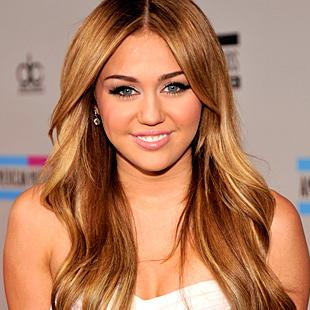
\includegraphics[width=.8\linewidth]{Graphics/vorher}
  \caption{vorher}
  \label{fig:fig1.1}
\end{subfigure}%
\begin{subfigure}{.5\textwidth}
  \centering
  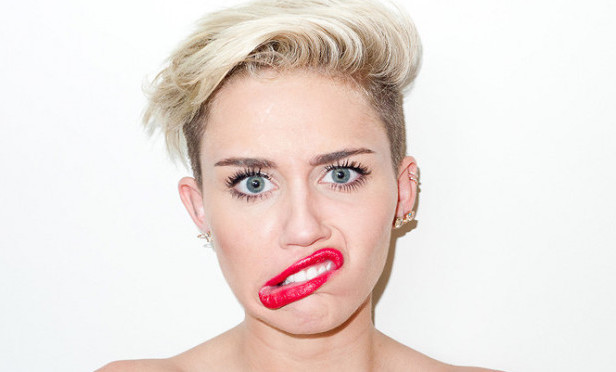
\includegraphics[width=.8\linewidth]{Graphics/nachher}
  \caption{nachher}
  \label{fig:fig1.2}
\end{subfigure}
\captionsetup{justification=raggedright,singlelinecheck=false}
\caption{plots of.... plots of.... plots of.... plots of.... plots of.... plots of.... plots of.... plots of.... plots of....}
\label{fig:fig}
\end{figure}
Nec vero habere virtutem satis est quasi artem aliquam nisi utare; etsi ars quidem cum ea non utare scientia tamen ipsa teneri potest, virtus in usu sui tota posita est; usus autem eius est maximus civitatis gubernatio, et earum ipsarum rerum quas isti in angulis personant, reapse non oratione perfectio. nihil enim dicitur a philosophis, quod quidem recte honesteque dicatur, quod ab iis partum confirmatumque sit, a quibus civitatibus iura discripta sunt. unde enim pietas, aut a quibus religio? unde ius aut gentium aut hoc ipsum civile quod dicitur? unde iustitia fides aequitas? unde pudor continentia fuga turpi<tu>dinis adpetentia laudis et honestatis? unde in laboribus et periculis fortitudo? nempe ab iis qui haec disciplinis informata alia moribus confirmarunt, sanxerunt autem alia legibus. 

\section{A section for tables}
An now another table in Tab.~(\ref{tab:tab2}). \\ \\ 
\begin{table*}[t] %t-top, b-bottom, h-in this place
  \centering
    \setlength\tabcolsep{1.5ex}
  \begin{tabular*}{\textwidth}{*{9}{c}}
    \hline \vspace{-2.5mm} \\
      & & && \multicolumn{2}{c}{ Schiller-Neumann }  && 
     \multicolumn{2}{c}{ ISO VG 46 } \\ \cline{5-6} \cline{8-9} \vspace{-2mm} \\ 
     \shortstack{$Q_\s{O}$ \\ $[l/min]$} & Design & \shortstack{$\alpha_\s{out}$ Exp \\ $[-]$} && \shortstack{$\alpha_\s{out}$ Sim \\ $[-]$} & \shortstack{Rel. Error \\ $[\%]$} && \shortstack{$\alpha_\s{out}$ Sim \\ $[-]$} & \shortstack{Rel. Error \\ $[\%]$} \vspace{1.5mm} \\
    \hline \vspace{-1.5mm} \\ 
    20 & 1. & 5.327E-4  && 8.347E-3 	& 990 	&& 7.661E-4 	& 44 \\
    30 & 1. & 1.236E-3  && 3.036E-2 	& 2260 	&& 1.286E-3 	& 4 \\
    50 & 1. & 2.368E-3  && 4.215E-2	    & 1542 	&& 2.567E-3 	& 8 \\
    70 & 1. & 4.746E-3  && 2.613E-2 	& 426 	&& 4.972E-3 	& 5 \\
    87 & 1. & 4.754E-3  && 2.280E-2 	& 347 	&& 5.097E-3 	& 7 \\
    70 & 2. & 1.416E-3  && 2.842E-3 	& 76.0 	&& 1.613E-3 	& 14 \\
    70 & 3. & 2.013E-3  && 1.241E-2 	& 440 	&& 2.297E-3 	& 14 \\
    70 & 4. & 1.228E-3  && 2.850E-3 	& 123 	&& 1.279E-3 	& 4 \\
    \hline
  \end{tabular*}
\captionsetup{justification=raggedright,singlelinecheck=false}
\caption{ Comparison of the drag correlations. Simulation results}
\label{tab:tab1}
\end{table*}
\lipsum[1-4]
\begin{table}[h]
\begin{center}
\setlength\tabcolsep{10ex}
\begin{tabular}{c c c}
%& & \\ % put some space after the caption
\hline
Name & Forces & Expression\\
\hline \\ [-4mm]
$\displaystyle Re$ & $\displaystyle \frac{F_\s{i}}{F_\s{\mu}}$  & $\displaystyle \frac{\rho_\s{O} v_\s{b} d}{\mu_\s{o}}$ \\ [2ex]
$\displaystyle Eo$ &  $\displaystyle \frac{F_\s{b}}{F_\s{\sigma}}$ & $\displaystyle \frac{(\rho_\s{o} - \rho_\s{A}) g d^2}{\sigma}$ \\[2ex]
$\displaystyle Mo$ & $\displaystyle \frac{F_\s{\mu}^4 F_\s{b}}{F_\s{\sigma}^3 F_\s{i}^2 }$ & $\displaystyle \frac{g \mu_\s{o}^4 (\rho_\s{o} - \rho_\s{a})}{\rho_\s{o}^2 \sigma^3}$ \\[2ex]
\hline
\end{tabular}
\end{center}
\captionsetup{justification=raggedright,singlelinecheck=false}
\caption{Dimensionless gruops}
\label{tab:tab2}
\end{table}





\begin{appendices}
\chapter{Appendix}
 \lipsum[1-8]
\end{appendices}

%\renewcommand\thechapter{\Alph{chapter}}
%\chapter{Appendix}
 \lipsum[1-8]
%\addcontentsline{toc}{chapter}{Appendix}

%Print list of figures and add to toc
\listoffigures
\addcontentsline{toc}{chapter}{List of Figures}

%Print list of tables and add to toc
\listoftables
\addcontentsline{toc}{chapter}{List of Tables}

\bibliography{dissertationTemplate}
\addcontentsline{toc}{chapter}{Bibliography}

\begin{cv}
\vspace{15ex}\textbf{\Large Pers\"onliche Daten}\vspace{1ex}
\begin{labeling}{\hspace{15em}}
	\item [Name] Marcus Tullius Cicero
	\item [Geburtsdatum] 03.01.107 v.Chr.
	\item [Geburtsort] Arpino
	\item [Familienstand] Verheiratet
\end{labeling}
\null\vspace{2ex}\textbf{\Large Schulausbildung}\vspace{1ex}
\begin{labeling}{\hspace{15em}}
	\item [08/103 -- 06/99 v. Chr.] Epische Grundschule
\end{labeling}
\null\vspace{2ex}\textbf{\Large Studium}\vspace{1ex}
\begin{labeling}{\hspace{15em}}
	\item [10/90 -- 09/86 v. Chr.] Studium da irgendwo
\end{labeling}
\null\vspace{2ex}\textbf{\Large Berufspraxis}\vspace{1ex}
\begin{labeling}{\hspace{15em}}
	\item [10/86 -- 12/43 v. Chr.] Redner/Politiker/Anwalt/Schriftsteller
\end{labeling}
\end{cv}

\end{document}